\section{Untersuchung der Kinematik}
Der erste Schritt in der Modellbildung besteht in der Definition der Bezugssystem, welche zur Beschreibung der Systembewegung dienen. Der Ausgangspunkt ist das Inertialsystem $A$, welches durch die drei Einheitsvektoren $\bs{a}_1$, $\bs{a}_2$ und $\bs{a}_3$ definiert wird. Das Würfelgehäuse verfügt über drei rotatorische Freiheitsgrade, welche durch die Winkel $\varphi_1$, $\varphi_2$ und $\varphi_3$ beschrieben werden. 

\begin{figure}[!h]
\centering
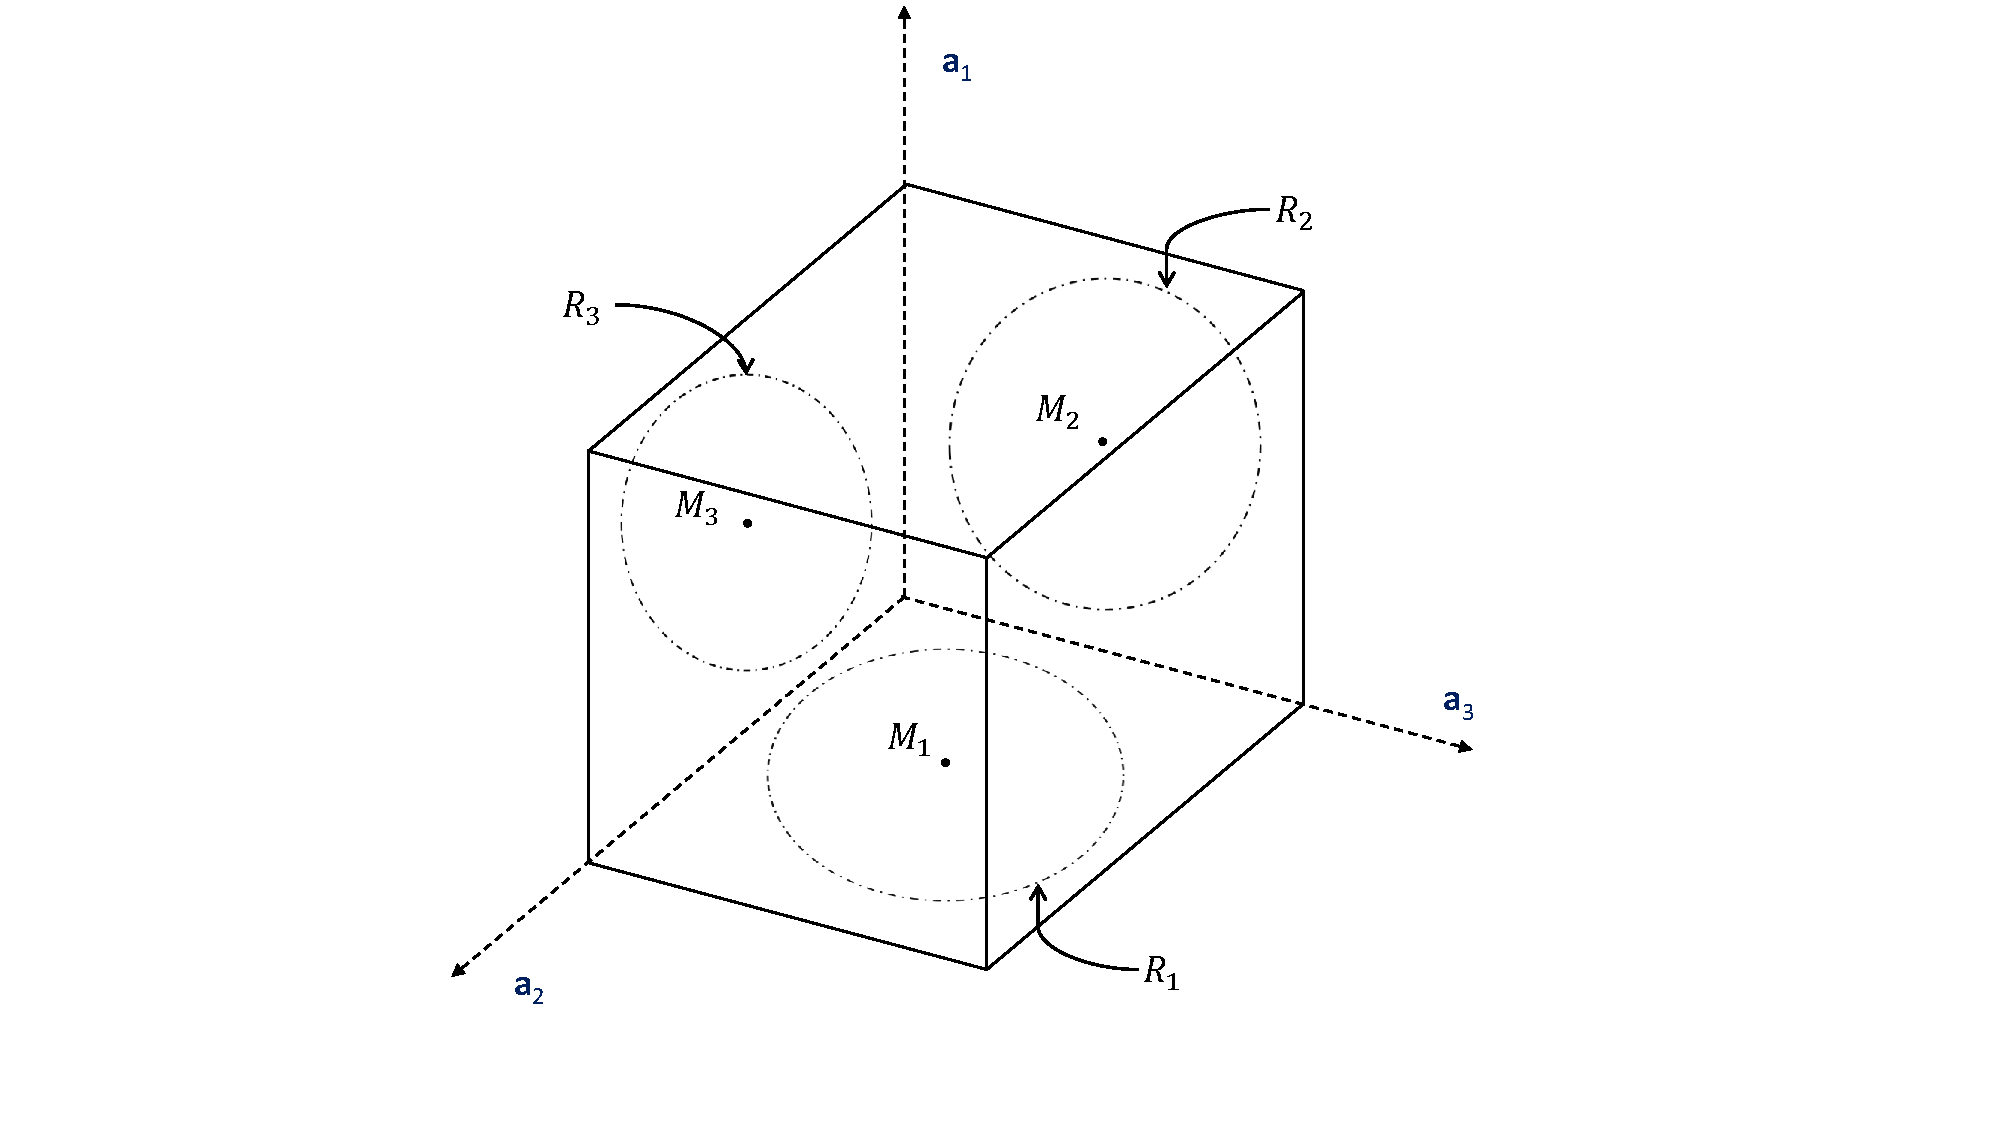
\includegraphics[width=\linewidth, trim={3cm 1.5cm 4cm 0cm}, clip]{img/MechAufbau3D}
\caption{Mechanischer Aufbau der Würfelseite, Quelle: eigene Darstellung}
\end{figure}

Durch die Rotation des Würfels um den Winkel $\varphi_1$ in Richtung des Vektors $\bs{a}_1$ entsteht das Hilfsbezugssystem $B$, das durch die Einheitsvektoren $\bs{b}_1$, $\bs{b}_2$ und $\bs{b}_3$ aufgespannt wird.
\begin{equation}
\presuper{A}{\bs{v}} = \presuper{B}{\Big( \pMat{A}{B} \cdot \presuper{A}{\bs{v}}\Big)} = \presuper{B}{\bs{v}} \hspace{35pt} \vert \hspace{15pt} \pMat{A}{B} = \begin{pmatrix}
1 & 0 & 0 \\ 0 & c_{\varphi_1} & s_{\varphi_1} \\ 0 & -s_{\varphi} & c_{\varphi_1}
\end{pmatrix}
\end{equation}
Die Rotation um den Winkel $\varphi_2$ in Richtung des Vektors $\bs{b}_2$ führt zu dem zweiten Hilfsbezugssystem $C$ mit den drei Einheitsvektoren $\bs{c}_1$, $\bs{c}_2$ und $\bs{c}_3$.
\begin{equation}
\presuper{B}{\bs{v}} = \presuper{C}{\Big( \pMat{B}{C} \cdot \presuper{B}{\bs{v}}\Big)} = \presuper{C}{\bs{v}} \hspace{35pt} \vert \hspace{15pt} \pMat{B}{C} = \begin{pmatrix}
c_{\varphi_2} & 0 & -s_{\varphi_2} \\ 0 & 1 & 0 \\ s_{\varphi_2} 0 c_{\varphi_2}
\end{pmatrix}
\end{equation}
Die letzte Rotation des Würfels in Richtung von $\bs{c}_3$ um den Winkel $\varphi_3$ führt zu dem körperfesten Bezugssystem $K$, welches durch die drei Vektoren $\bs{k}_1$, $\bs{k}_2$ und $\bs{k}_3$ definiert ist.
\begin{equation}
\presuper{C}{\bs{v}} = \presuper{K}{\Big( \pMat{C}{K} \cdot \presuper{C}{\bs{v}}\Big)} = \presuper{K}{\bs{v}} \hspace{35pt} \vert \hspace{15pt} \pMat{C}{K} = \begin{pmatrix}
c_{\varphi_3} & s_{\varphi_3} & 0 \\ -s_{\varphi_3} & c_{\varphi_3} & 0 \\ 0 & 0 & 1
\end{pmatrix}
\end{equation}
Hier sei angemerkt, dass es sich bei den Bezugssystem $B$ und $C$ um theoretische Konstrukte handelt, für die kein physisches Gegenstück existiert. Sie werden lediglich als Hilfsmittel zur Beschreibung des Systems verwendet.

Durch die Rotation der Schwungmassen besitzt das System drei weitere Freiheitsgrade, welche von den Winkeln $\psi_1$, $\psi_2$ und $\psi_3$ beschrieben werden. Somit entstehen drei weitere Bezugssysteme, deren Vektorbasen jeweils an den Schwungmassen fixiert sind. Allerdings spielen diese keine weitere Rolle, da es sich bei den Winkeln $\psi_i$ um zyklische Koordinaten handelt. Das heißt, dass der Impuls des Systems nicht von der Ausrichtung der Schwungmassen abhängt. Lediglich die Winkelgeschwindigkeiten $\dot{\psi}_i$ beeinflussen auf Grund der Reibung das System.

Die Position und Ausrichtung des Systems wird von den sechs Winkeln $\varphi_i$ und $\psi_i$ vollständig beschrieben. Deshalb werden diese als generalisierte Koordinaten $q_i$ definiert.
\begin{equation}
q_i = \varphi_i \hspace{35pt} q_j = \psi_i \hspace{35pt} (i=1,2,3; j=4,5,6)
\end{equation}
Mit Hilfe der Bezugssysteme und generalisierten Koordinaten können nun die Winkelgeschwindigkeit des Würfels $\vel{A}{\omega}{K}$ und der Schwungmassen $\vel{A}{\omega}{R_i}$ bestimmt werden. Diese ergeben sich aus der Addition der relativen Rotationsgeschwindigkeiten der Bezugssysteme zueinander.
\begin{equation}
\begin{split}
\vel{A}{\omega}{K} &= \vel{A}{\omega}{B}+\vel{B}{\omega}{C}+\vel{C}{\omega}{K} = \vecBS{A}{\dot{\varphi}_1}{0}{0} + \vecBS{B}{0}{\dot{\varphi}_2}{0} + \vecBS{C}{0}{0}{\dot{\varphi}_3} \\
&= \vecBS{K}
{\dot{\varphi}_2\cdot s_{\varphi_3} + \dot{\varphi}_1 \cdot c_{\varphi_2}\cdot c_{\varphi_3}}
{\dot{\varphi}_2\cdot c_{\varphi_3} - \dot{\varphi}_1 \cdot c_{\varphi_2}\cdot s_{\varphi_3}}
{\dot{\varphi}_3 + \dot{\varphi}_1\cdot s_{\varphi_2}}
\end{split}
\end{equation}
Die Winkelgeschwindigkeiten der Schwungmassen $\vel{K}{\omega}{R_i}$ relativ zu dem Würfel entsprechen der ersten Ableitung der Winkel $\psi_i$. Mit Hilfe des Additionstheorems für Winkelgeschwindigkeiten kann daraus auch die absolute Winkelgeschwindigkeit der Schwungmassen $\vel{A}{\omega}{R_i}$ berechnet werden.
\begin{equation}
\vel{K}{\omega}{R_1} = \vecBS{K}{\dot{\psi}_1}{0}{0} \hspace{35pt}
\vel{K}{\omega}{R_2} = \vecBS{K}{0}{\dot{\psi}_2}{0} \hspace{35pt}
\vel{K}{\omega}{R_3} = \vecBS{K}{0}{0}{\dot{\psi}_3} 
\end{equation}
\begin{equation}
\vel{A}{\omega}{R_i} = \vel{A}{\omega}{K} + \vel{K}{\omega}{R_i} \hspace{35pt} (i=1,2,3)
\end{equation}
Im nächsten Schritt werden die absoluten Geschwindigkeiten der Teilsysteme in Komponenten zerlegt, welche sich aus den generalisierten Geschwindigkeiten $u_i$ und partiellen Geschwindigkeiten $\vel{A}{\omega}{j}_i$ zusammensetzen. Hierfür müssen zu nächst die generalisierten Geschwindigkeiten $u_i$ definiert werden. An dieser Stelle sei erwähnt, dass die Definition der generalisierten Geschwindigkeiten die Form der resultierenden Bewegungsgleichungen stark beeinflusst. Das letztendliche Ziel bei der Wahl der generalisierten Geschwindigkeiten ist es möglichst einfache Bewegungsgleichungen zu erhalten. Dies kann, nach einer Heuristik von Kane, erreicht werden, in dem die generalisierten Geschwindigkeiten so gewählt werden, dass die Geschwindigkeiten der Körper im Intertialsystem auf möglichst einfache Terme reduziert werden können. In diesem Anwendungsfall werden nach diesem Ansatz die folgenden generalisierten Geschwindigkeiten gewählt.
\begin{equation}
\begin{split}
u_1 &= \dot{\varphi}_2\cdot s_{\varphi_3} + \dot{\varphi}_1\cdot c_{\varphi_2}\cdot c_{\varphi_3} \\
u_2 &= \dot{\varphi}_2\cdot c_{\varphi_3} - \dot{\varphi}_1\cdot c_{\varphi_2}\cdot s_{\varphi_3} \\
u_3 &= \dot{\varphi}_3 + \dot{\varphi}_1\cdot s_{\varphi_2} \\
u_4 &= \dot{\varphi}_2\cdot s_{\varphi_3} + \dot{\varphi}_1\cdot c_{\varphi_2}\cdot c_{\varphi_3} + \dot{\psi}_1 \\
u_5 &= \dot{\varphi}_2\cdot c_{\varphi_3} - \dot{\varphi}_1\cdot c_{\varphi_2}\cdot s_{\varphi_3} + \dot{\psi}_2 \\
u_6 &= \dot{\varphi}_3 + \dot{\varphi}_1\cdot s_{\varphi_2} + \dot{\psi}_3
\end{split}
\end{equation}
Mit diesen Definitionen können die Winkelgeschwindigkeiten der Körper im A in die folgende Form gebracht werden.
\begin{equation}
\vel{A}{\omega}{K} = \vecBS{K}{u_1}{u_2}{u_3}, \vel{A}{\omega}{R1} = \vecBS{K}{u_4}{u_2}{u_3}, \vel{A}{\omega}{R2} = \vecBS{K}{u_1}{u_5}{u_3}, \vel{A}{\omega}{R3} = \vecBS{K}{u_1}{u_2}{u_6}
\end{equation}
Die Einführung der generalisierten Geschwindigkeiten führt einerseits zu einem stark vereinfachten Ausdruck der absoluten Winkelgeschwindigkeiten. Andererseits können dadurch auch die partiellen Geschwindigkeiten $\vel{A}{\omega}{j}_i$ in einfachen Termen ausgedrückt werden, wie die folgenden Gleichungen zeigen. Dadurch werden die folgenden Schritte der Modellbildung zunehmend erleichtert. 
\begin{align}
\vel{A}{\omega}{K} &= u_1 \cdot \bs{k}_1 + u_2 \cdot \bs{k}_2 + u_3 \cdot \bs{k}_3 &\rArrow &\vel{A}{\omega}{K}_1 = \bs{k}_1, \vel{A}{\omega}{K}_2 = \bs{k}_2, \vel{A}{\omega}{K}_3 = \bs{k}_3 \\
& & &\vel{A}{\omega}{K}_4 = 0, \vel{A}{\omega}{K}_5 = 0, \vel{A}{\omega}{K}_6 = 0 
\\
\vel{A}{\omega}{R_1} &= u_4 \cdot \bs{k}_1 + u_2 \cdot \bs{k}_2 + u_3 \cdot \bs{k}_3 &\rArrow 
&\vel{A}{\omega}{K}_1 = 0, \vel{A}{\omega}{K}_2 = \bs{k}_2, \vel{A}{\omega}{K}_3 = \bs{k}_3 \\
& & &\vel{A}{\omega}{K}_4 = \bs{k}_1, \vel{A}{\omega}{K}_5 = 0, \vel{A}{\omega}{K}_6 = 0 
\\
\vel{A}{\omega}{R_2} &= u_1 \cdot \bs{k}_1 + u_5 \cdot \bs{k}_2 + u_3 \cdot \bs{k}_3&\rArrow 
&\vel{A}{\omega}{K}_1 = \bs{k}_1, \vel{A}{\omega}{K}_2 = 0, \vel{A}{\omega}{K}_3 = \bs{k}_3 \\
& & &\vel{A}{\omega}{K}_4 = 0, \vel{A}{\omega}{K}_5 = \bs{k}_2, \vel{A}{\omega}{K}_6 = 0 
\\
\vel{A}{\omega}{R_3} &= u_1 \cdot \bs{k}_1 + u_2 \cdot \bs{k}_2 + u_6 \cdot \bs{k}_3&\rArrow 
&\vel{A}{\omega}{K}_1 = \bs{k}_1, \vel{A}{\omega}{K}_2 = \bs{k}_2, \vel{A}{\omega}{K}_3 = 0 \\
& & &\vel{A}{\omega}{K}_4 = 0, \vel{A}{\omega}{K}_5 = 0, \vel{A}{\omega}{K}_6 = \bs{k}_3
\end{align}
Die Unterteilung der absoluten Winkelgeschwindigkeiten in generalisierte und partielle Geschwindigkeiten ermöglicht den Übergang der vektoriellen Rechnung in die skalare. Die generalisierten Geschwindigkeiten geben als skalare Größen den Betrag der Bewegung in die Richtung der jeweiligen Freiheitsgrade wieder. Wobei die partiellen Geschwindigkeiten diese Richtung der Freiheitsgrade als vektorielle Größe mit Bezug auf das körperfeste Bezugssystem $K$ wiedergeben. Dadurch können weitere Vektoren wie z.B. Trägheitsmomente durch die Skalarmultiplikation mit den partiellen Geschwindigkeiten in die Richtung der Freiheitsgrade abgebildet werden.